\documentclass[11pt,a4paper]{article}

% ------------------------- Preamble -------------------------
\usepackage[T1]{fontenc}
\usepackage[utf8]{inputenc}
\usepackage{lmodern}
\usepackage[english]{babel}
\usepackage{csquotes}
\usepackage{amsmath}
\usepackage{booktabs}
\usepackage{siunitx}
\usepackage{graphicx}
\usepackage{tikz}
\usetikzlibrary{arrows.meta}
\usepackage[margin=2.5cm]{geometry}
\usepackage{caption}
\captionsetup{font=small,labelfont=bf,skip=6pt}
\usepackage[backend=biber,style=apa]{biblatex}
\addbibresource{refs.bib}
\usepackage[colorlinks=true,linkcolor=blue!60!black,citecolor=blue!60!black,urlcolor=blue!60!black]{hyperref}
\usepackage{microtype}

\sisetup{detect-family=true}

\title{\textbf{Synthetic Council: Can AI Agents Estimate Consensus\\ in the ECB Governing Council?}}
\author{Luigi Palumbo \and Sophia Kazinnik}
\date{October 2026}

% ------------------------- Document -------------------------
\begin{document}
\maketitle

\begin{abstract}
\noindent
We simulate the European Central Bank's Governing Council with large language model (LLM) agents and ask two questions: can the simulation estimate the degree of consensus inside the committee, and does country-specific economic information change that consensus? For each of 94 monetary policy meetings from 2015 to 2026, 21--27 agents---conditioned on verified member profiles, true-vintage macroeconomic data, ECB staff projections, and their own recent speeches---deliberate around the Chief Economist's proposal, extracted verbatim from the monetary policy accounts. A two-arm design varies only the information set: governors in the treatment arm additionally receive a country macro annex. The simulated council tracks real decisions closely (95.7--97.9\% direction accuracy, robust across two different generators), but the country annex leaves consensus unchanged: the treatment effect is a robust null (between $-1.4$ and $+0.9$ percentage points, opposite signs across generators). Estimated decision modes are above chance yet biased toward unanimity and sensitive to the generator. Synthetic councils currently forecast decisions well, but are not yet a measurement-grade instrument for consensus.
\end{abstract}

\section{Introduction}\label{sec:intro}

How much agreement reigns inside the ECB Governing Council at the moment a rate decision is taken? The question matters. \textcite{riboni2010committee} estimate that a consensus protocol---requiring a supermajority for a policy change---fits the ECB's interest-rate decisions better than chairman-dictatorship or simple-majority rules, so the distribution of views, not just the median, drives policy. Market participants price it: central bank tone, which reflects the dispersion of views within the committee, moves interest rates and predicts future decisions \parencite{hubert2019tone}. Yet the object itself is essentially unobserved in real time. The ECB publishes no individual votes, and the monetary policy accounts arrive weeks later as an edited summary: minutes are by construction a shortened representation of a broader discussion, and systematically omit information about the level of agreement among members \parencite{apel2021disclose}.

This paper proposes and evaluates a measurement strategy based on generative AI: build a \emph{synthetic council}---one LLM agent per real member, each conditioned on the information the member actually had and on a documented profile of the member's background and stated views---and read the committee's degree of consensus off the simulated deliberation. The exercise is deliberately anchored to the historical record: every simulated meeting opens with the Chief Economist's actual policy proposal, extracted verbatim from the accounts, and the roster, voting rights, and outcome ground truths all come from the same source. The simulation is therefore not asked to imagine an agenda; it is asked to deliberate a real one.

We use the simulation to answer two research questions. First, can AI-agent deliberation \emph{estimate consensus}: do the decisions it produces match the real ECB decisions, and does its characterization of the decision mode (unanimity, consensus, or majority) match the classification derivable from the accounts? Second, does \emph{country-specific information} change estimated consensus? National governors sit on the Council alongside the Executive Board, and a substantial literature argues their positions reflect national conditions---governors from high-debt countries tilt dovish \parencite{heinemann2021fiscal}, national background predicts Council behavior \parencite{badinger2013national}, and in the FOMC analogue, district presidents dissent in line with local unemployment \parencite{bobrov2024regional}. Our two-arm experiment tests the informational channel directly: governors in the treatment arm receive an additional country macro annex, and the annex is the \emph{only} difference between arms.

Three findings emerge. First, the apparatus is valid where it is easiest to check: the simulated council's decisions match the direction of real ECB decisions in 95.7--97.9\% of meetings, and simulated decision stances agree across two entirely different generators (GLM-5.3-Flash and Muse-Spark) in 95.7--97.9\% of meetings. Anchoring deliberation on the real proposal dominates everything else. Second, the country annex is a robust null: mean within-meeting alignment with the simulated decision moves by $+0.9$ percentage points under Muse-Spark ($p = 0.92$) and $-1.4$ points under GLM ($p = 0.08$)---opposite signs, each economically negligible, and never distinguishable from zero at conventional levels in the direction either generator suggests. Third, consensus itself is the hard part: decision-mode estimates beat an always-unanimity benchmark (43--47 vs.\ 35 of 94 meetings) but err systematically toward unanimity---the synthetic council over-converges relative to the real one---and mode labels agree across generators in barely 60\% of meetings. A single-generator reading would have tempted a ``small negative effect'' claim; the replication exposes it as an apparatus artifact.

The paper contributes a design template for committee simulation: verbatim anchoring on real proposals, true-vintage information sets, a treatment that varies only the information set, and a cross-generator replication discipline in which the two experiments are never pooled. Section~\ref{sec:related} situates the work. Section~\ref{sec:design} describes data, simulation, and measurement (Figure~\ref{fig:pipeline}). Section~\ref{sec:results} presents results, and Section~\ref{sec:discussion} discusses what the exercise can and cannot yet measure.

\section{Related work}\label{sec:related}

\subsection{LLM agents simulating humans and committees}

Generative agents built on LLMs---endowed with personas, memory, and reflection---produce behavior that is plausible at the individual level and structured at the population level \parencite{park2023generative}, and the approach has spread across social simulation \parencite{gao2024large}. A growing validation literature asks when such agents actually track the humans they stand for: preregistered programs ground agents in interviews with specific individuals \parencite{park2024interviews}, richer profiling modules improve persona fidelity \parencite{cerqueira2025motif}, and whole-society simulations are evaluated against real-world outcomes, with documented alignment failures \parencite{hou2025vacsim}. In economics, LLM personas replicate the cross-section of the Survey of Professional Forecasters \parencite{hansen2025spf}, LLMs forecast macroeconomic series competitively \parencite{carriero2024macro}, and ChatGPT classifies FOMC communication on a hawkish--dovish scale at human parity \parencite{hansen2024chatgpt}.

Closest to us, \textcite{kazinnik2025fomc} simulate the FOMC with a multi-agent system seeded by member priors from real-time data and member profiles, and \textcite{seok2024minifed} organize LLM agents into a five-stage meeting of discussion, persuasion, and voting. Our design differs in three ways. We anchor every meeting on the verbatim Chief Economist proposal rather than an inferred agenda; we target the committee's \emph{degree of consensus} rather than the level of the rate; and we embed a randomized-information treatment---identical in every respect except one table---with a pre-specified paired analysis and a full replication under a different generator.

\subsection{Consensus and heterogeneity in monetary policy committees}

That committees, not individuals, set monetary policy is standard; how they aggregate preferences is not. \textcite{riboni2010committee} show a consensus protocol fits five committees including the ECB best; former Governing Council members describe a strong consensus-seeking culture \parencite{ehrmann2023communication}. Composition and background shape positions: national representation and home-country characteristics matter in the ECB Council \parencite{badinger2013national, heinemann2021fiscal}, and enlargement reshaped its voting power \parencite{fahrholz2004emu}. For the FOMC, lifetime inflation experiences and cohort background predict hawkishness \parencite{malmendier2017hawks, bordo2018perceived}, and regional conditions move district presidents' votes \parencite{bobrov2024regional}. Where individual votes are published, reaction functions recover preference heterogeneity \parencite{jung2012voting}; where they are not, researchers infer dispersion from text---tone, hawkishness dictionaries, and machine-learning agreement measures \parencite{tobback2017between, hubert2019tone, apel2021disclose}. Our experiment connects the two strands: it asks whether the national-information channel that the heterogeneity literature documents can be detected \emph{inside} a simulated Council, by varying exactly that information.

\section{Data and experimental design}\label{sec:design}

Figure~\ref{fig:pipeline} summarizes the pipeline from raw sources to measured outcomes; this section walks through it.

\begin{figure}[t]
\centering
% Figure 1: end-to-end pipeline of the synthetic-council simulation.
% Included from main.tex inside a figure environment (A4 portrait, full text width).
% Natural size: 16cm wide (= \textwidth with a4paper + 2.5cm margins), ~13.2cm tall.
% No scaling: fonts render at nominal size (\footnotesize = 9pt at 11pt base).

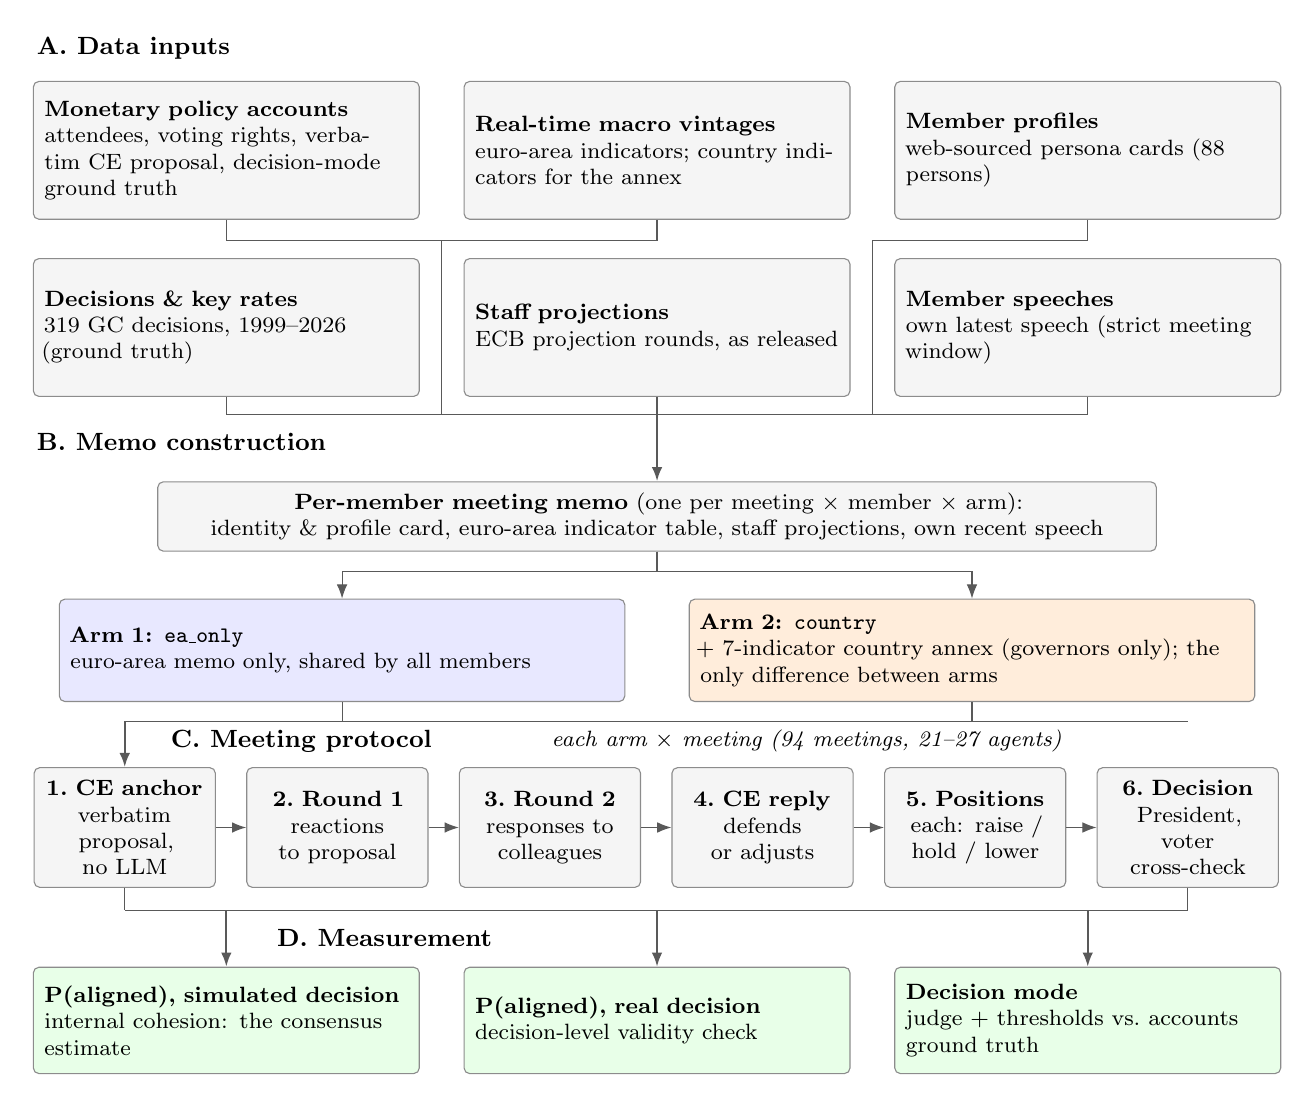
\begin{tikzpicture}[
  font=\footnotesize,
  box/.style={draw=black!45, rounded corners=2pt, align=left, inner sep=4pt},
  databox/.style={box, fill=black!4, text width=4.62cm, minimum height=1.75cm},
  memobox/.style={box, fill=black!4, text width=12.4cm, align=center},
  armbox/.style={box, text width=6.9cm, minimum height=1.3cm},
  stepbox/.style={box, fill=black!4, text width=2.02cm, align=center, minimum height=1.52cm},
  outbox/.style={box, text width=4.62cm, minimum height=1.35cm},
  bandlabel/.style={font=\small\bfseries, anchor=west},
  ln/.style={black!65},
  fl/.style={-{Latex[length=1.8mm]}, black!65},
  flt/.style={fl, thick},
]

% ---------------- Band A: data inputs (two rows of three) ----------------
\node[bandlabel] at (-8.0, 1.0) {A.~Data inputs};
\node[databox] (a1) at (-5.47, -0.3)
  {\textbf{Monetary policy accounts}\\ attendees, voting rights, verbatim CE proposal, decision-mode ground truth};
\node[databox] (a2) at (0.0, -0.3)
  {\textbf{Real-time macro vintages}\\ euro-area indicators; country indicators for the annex};
\node[databox] (a3) at (5.47, -0.3)
  {\textbf{Member profiles}\\ web-sourced persona cards (88 persons)};
\node[databox] (a4) at (-5.47, -2.55)
  {\textbf{Decisions \& key rates}\\ 319 GC decisions, 1999--2026 (ground truth)};
\node[databox] (a5) at (0.0, -2.55)
  {\textbf{Staff projections}\\ ECB projection rounds, as released};
\node[databox] (a6) at (5.47, -2.55)
  {\textbf{Member speeches}\\ own latest speech (strict meeting window)};

% ---------------- Band B: memo construction ----------------
\node[bandlabel] at (-8.0, -4.0) {B.~Memo construction};
\node[memobox] (memo) at (0.0, -4.95)
  {\textbf{Per-member meeting memo} (one per meeting $\times$ member $\times$ arm):\\
   identity \& profile card, euro-area indicator table, staff projections, own recent speech};
\node[armbox, fill=blue!9] (ea) at (-4.0, -6.65)
  {\textbf{Arm 1: \texttt{ea\_only}}\\ euro-area memo only, shared by all members};
\node[armbox, fill=orange!14] (co) at (4.0, -6.65)
  {\textbf{Arm 2: \texttt{country}}\\ $+$ 7-indicator country annex (governors only); the only difference between arms};

% input bus: row-2 boxes drop straight down; row-1 boxes route through the
% column gaps (x = +-2.735) into the same bus
\draw[ln] (a1.south) -- (-5.47,-1.45) -- (-2.735,-1.45) -- (-2.735,-3.65);
\draw[ln] (a2.south) -- (0,-1.45) -- (-2.735,-1.45);
\draw[ln] (a3.south) -- (5.47,-1.45) -- (2.735,-1.45) -- (2.735,-3.65);
\draw[ln] (-5.47,-3.65) -- (5.47,-3.65);
\draw[ln] (a4.south) -- (-5.47,-3.65);
\draw[ln] (a5.south) -- (0,-3.65);
\draw[ln] (a6.south) -- (5.47,-3.65);
\draw[flt] (0,-3.65) -- (memo.north);
\draw[fl] (memo.south) -- ++(0,-0.25) -| (ea.north);
\draw[fl] (memo.south) -- ++(0,-0.25) -| (co.north);

% ---------------- Band C: meeting protocol (chain of six) ----------------
\node[stepbox] (s1) at (-6.76, -8.9) {\textbf{1.~CE anchor}\\ verbatim proposal, no LLM};
\node[stepbox] (s2) at (-4.06, -8.9) {\textbf{2.~Round 1}\\ reactions to proposal};
\node[stepbox] (s3) at (-1.36, -8.9) {\textbf{3.~Round 2}\\ responses to colleagues};
\node[stepbox] (s4) at (1.34, -8.9) {\textbf{4.~CE reply}\\ defends or adjusts};
\node[stepbox] (s5) at (4.04, -8.9) {\textbf{5.~Positions}\\ each: raise / hold / lower};
\node[stepbox] (s6) at (6.74, -8.9) {\textbf{6.~Decision}\\ President, voter cross-check};
\draw[fl] (s1) -- (s2);
\draw[fl] (s2) -- (s3);
\draw[fl] (s3) -- (s4);
\draw[fl] (s4) -- (s5);
\draw[fl] (s5) -- (s6);
\draw[ln] (-6.76,-7.55) -- (6.74,-7.55);
\draw[ln] (ea.south) -- (-4.0,-7.55);
\draw[ln] (co.south) -- (4.0,-7.55);
\draw[flt] (-6.76,-7.55) -- (s1.north);
\node[bandlabel] at (-6.3,-7.8) {C.~Meeting protocol};
\node[font=\footnotesize\itshape] at (1.9,-7.8) {each arm $\times$ meeting (94 meetings, 21--27 agents)};

% ---------------- Band D: measurement ----------------
\node[outbox, fill=green!9] (m1) at (-5.47, -11.35)
  {\textbf{P(aligned), simulated decision}\\ internal cohesion: the consensus estimate};
\node[outbox, fill=green!9] (m2) at (0.0, -11.35)
  {\textbf{P(aligned), real decision}\\ decision-level validity check};
\node[outbox, fill=green!9] (m3) at (5.47, -11.35)
  {\textbf{Decision mode}\\ judge $+$ thresholds vs.\ accounts ground truth};
\draw[ln] (-6.76,-9.95) -- (6.74,-9.95);
\draw[ln] (s1.south) -- (-6.76,-9.95);
\draw[ln] (s6.south) -- (6.74,-9.95);
\draw[flt] (-5.47,-9.95) -- (m1.north);
\draw[flt] (0,-9.95) -- (m2.north);
\draw[flt] (5.47,-9.95) -- (m3.north);
\node[bandlabel] at (-4.95,-10.3) {D.~Measurement};

\end{tikzpicture}

\caption{The synthetic-council pipeline. Band A: data inputs collected from primary sources with no look-ahead (true-vintage macro data and staff projections as released at the time). Band B: one memo per meeting $\times$ member $\times$ arm; the country annex is the only difference between arms. Band C: the six-step meeting protocol run for each of the 94 meetings in each arm. Band D: per-member alignment probabilities (the consensus estimate), the validity check against real decisions, and decision-mode classification against the accounts ground truth.}
\label{fig:pipeline}
\end{figure}

\subsection{Data and anchoring}\label{sec:data}

The sample is the accounts era: 94 Governing Council monetary policy meetings from January 2015 to September 2026 for which the monetary policy accounts provide a usable anchor. Three extractions come from the accounts themselves. First, the roster: meeting-by-meeting attendance and voting rights (the accounts mark members without a voting right in a given month), matched to verified tenure records---2,417 meeting-member rows. Second, the anchor: the Chief Economist's policy proposal, extracted verbatim from the accounts narrative (96 proposals; 69 by deterministic pattern-matching, the remainder by supervised extraction flagged as such). Third, the ground truth for consensus: a two-stage classification of each meeting's decision mode---unanimity, consensus, or majority---first curating verbatim agreement/disagreement quotes from the accounts, then classifying the evidence against standard definitions; the accounts' own labels are never observed by the simulation. In the sample, the ground-truth margins are 35 unanimity, 39 consensus, and 20 majority meetings.

Agent information sets are built with a strict no-look-ahead discipline. The euro-area memo carries eight indicators (headline and core inflation, GDP growth, unemployment, industrial production, financial stress, and two confidence measures) taken from \emph{true vintages}---the data as actually available at the meeting date---plus the latest ECB staff projection round, released only from its publication month. Each member's profile card is built once from verified tenures, web-sourced background with archived sources, and a policy-orientation section distilled from the member's own speeches before the meeting (qualitative, in the spirit of \textcite{hansen2024chatgpt}); where a member gave a speech in the window between the previous and current meeting, the speech itself enters the memo. Real decisions and key rates (319 meetings, 1999--2026) provide the outcome ground truth.

\subsection{Memos and the two arms}\label{sec:memos}

Each of the roughly 5,000 (meeting $\times$ member) pairs receives a memo containing: the member's identity and profile card, the euro-area indicator table, the staff projections, and the member's own most recent qualifying speech. The experiment varies exactly one input. In the \texttt{ea\_only} arm, all members receive this shared memo. In the \texttt{country} arm, national governors additionally receive a country annex: a seven-indicator table (GDP growth, headline and core inflation, industrial production, unemployment, and two confidence measures) for their own country, drawn from the same vintage discipline. A file-level diff verifies that this annex is the only difference between arms; Executive Board memos are identical by construction. The design cleanly isolates the informational channel: if national conditions move governors' positions---the channel the heterogeneity literature emphasizes---the annex must move the simulated deliberation.

\subsection{The meeting protocol}\label{sec:protocol}

Each meeting $\times$ arm runs a six-step protocol with 21--27 agents (mean 24.9; the same roster in both arms). (1)~The Chief Economist's verbatim proposal opens the meeting; no LLM call is made. (2)~Round 1: every non-CE member reacts to the proposal, grounded in their memo and persona. (3)~Round 2: members respond to colleagues, seeing the transcript so far. The Chief Economist is silent during both rounds. (4)~The Chief Economist replies, defending, conceding, or adjusting. (5)~Every member states a final position ending with an explicit ``Position: raise/hold/lower'' line. (6)~The President formulates the decision; a deterministic cross-check records the modal final stance of voting-right members and flags disagreement.

\subsection{Outcome measures}\label{sec:outcomes}

A separate judge model scores each member's final statement against two references, returning $\text{P}(\text{aligned})$ for each: alignment with the \emph{simulated} decision and with the \emph{real} ECB decision (direction, size, and resulting rate levels). Our consensus estimate for meeting $m$ is the within-meeting mean
\[
C_m \;=\; \frac{1}{N_m} \sum_{i=1}^{N_m} p_i, \qquad p_i = \text{P}(\text{member } i \text{ aligned with the simulated decision}),
\]
which is high when final statements cohere with the decision the council itself took. The treatment effect is the paired difference $\Delta_m = C_m^{\texttt{country}} - C_m^{\texttt{ea\_only}}$, averaged over the 94 meetings, with an exact sign test and a bootstrap 95\% confidence interval. Decision validity is the share of meetings whose simulated stance matches the real decision's direction. The decision mode is measured two ways: (i)~the judge classifies the closing evidence with the same criteria used for the ground-truth extraction, making the comparison symmetric; (ii)~a deterministic aggregation of the $p_i$---unanimity if every member has $p_i \geq 0.85$; consensus if at least 70\% of members have $p_i \geq 0.5$ and none falls below 0.2; majority otherwise.

\subsection{Apparatus and replication discipline}\label{sec:apparatus}

Table~\ref{tab:apparatus} reports the two full experiments. The primary run uses GLM-5.3-Flash as the generator (temperature 0.7); the replication uses Muse-Spark; both use the same judge (Clef, a 27-billion-parameter decision model returning full probability distributions), the same prompts, arms, thresholds, and rosters, and the same 94 meetings---14,058 generator calls per experiment. We never pool the two experiments: the generator is part of the apparatus, held fixed within each experiment, and cross-generator statements are descriptive. Every LLM call is logged in per-meeting ledgers, so all measurement stages can be replayed without new generator calls.

\begin{table}[t]
\centering
\small
\caption{Apparatus and scale of the two experiments. Each experiment is a complete two-arm run over the same 94 meetings; the two are never pooled.}
\label{tab:apparatus}
\begin{tabular}{lcc}
\toprule
 & Experiment 1 (primary) & Experiment 2 (replication) \\
\midrule
Generator & GLM-5.3-Flash & Muse-Spark-816B \\
Sampling & temp.\ 0.7, low reasoning & temp.\ 0.7, heavy reasoning \\
Judge (alignment, modes) & Clef 27B (decisions API) & Clef 27B (decisions API) \\
Meetings $\times$ arms & $94 \times 2$ & $94 \times 2$ \\
Agents per meeting & 21--27 & 21--27 \\
Generator calls & 14,058 & 14,058 \\
Tokens (input / output) & 109.4M / 11.2M & 75.4M / 44.9M \\
Wall time & $\sim$9.5 h & $\sim$23.5 h \\
Cost & \$24.23 & $\approx$\$2 (promo tier) \\
\bottomrule
\end{tabular}
\end{table}

\section{Results}\label{sec:results}

\subsection{The synthetic council tracks real decisions}\label{sec:validity}

Across 94 meetings, the simulated decision matches the direction of the real ECB decision in 95.7\% of meetings under GLM (both arms) and 95.7--97.9\% under Muse (Table~\ref{tab:modes}, last column). The cross-generator comparison is sharper still: run with entirely different generators, the two synthetic councils produce the same decision stance in 95.7\% of \texttt{ea\_only} meetings and 97.9\% of \texttt{country} meetings, with disagreements concentrated in the close calls of 2019--2022. Whatever the deliberation model adds on top of the record, the combination of the verbatim proposal anchor and the shared euro-area information set pins the decision down almost mechanically. This is the floor of validity: an apparatus that could not reproduce decisions could not credibly measure the consensus behind them.

\subsection{Country information does not move estimated consensus}\label{sec:treatment}

Table~\ref{tab:treatment} and Figure~\ref{fig:delta} report the treatment effect. Under Muse-Spark, the country annex raises mean alignment with the simulated decision by $+0.0086$ (bootstrap 95\% CI $[-0.0065, +0.0262]$; exact sign test $p = 0.918$). Under GLM, the point estimate is $-0.0143$ (CI $[-0.0268, -0.0038]$; $p = 0.079$): the only confidence interval that excludes zero, but with the \emph{opposite sign} to the replication. Both point estimates are economically negligible---at most 1.5 percentage points on a base of 0.92--0.96---and the sign flips across generators whose baseline cohesion levels themselves differ (0.916--0.925 under Muse vs.\ 0.944--0.959 under GLM). Read together, the experiments deliver a robust null: within this design, handing governors their country's indicators neither systematically tightens nor loosens the simulated council.

\begin{table}[t]
\centering
\small
\caption{Treatment effect of the country annex on estimated consensus. $C$ is the within-meeting mean P(aligned with the simulated decision); $\Delta$ is the paired per-meeting difference (country $-$ \texttt{ea\_only}), $n = 94$ meetings. Bootstrap 95\% confidence intervals (10,000 resamples); $p$ from the exact sign test.}
\label{tab:treatment}
\begin{tabular}{llcccc}
\toprule
Experiment & Arm & $C$ & $\Delta$ mean & 95\% CI & $p$ \\
\midrule
GLM (primary) & \texttt{ea\_only}   & 0.9588 & $-0.0143$ & $[-0.0268,\, -0.0038]$ & 0.079 \\
             & \texttt{country}    & 0.9445 &           &                        &       \\
\addlinespace
Muse (replication) & \texttt{ea\_only} & 0.9164 & $+0.0086$ & $[-0.0065,\, +0.0262]$ & 0.918 \\
                   & \texttt{country}  & 0.9251 &           &                        &       \\
\bottomrule
\end{tabular}
\end{table}

\begin{figure}[t]
\centering
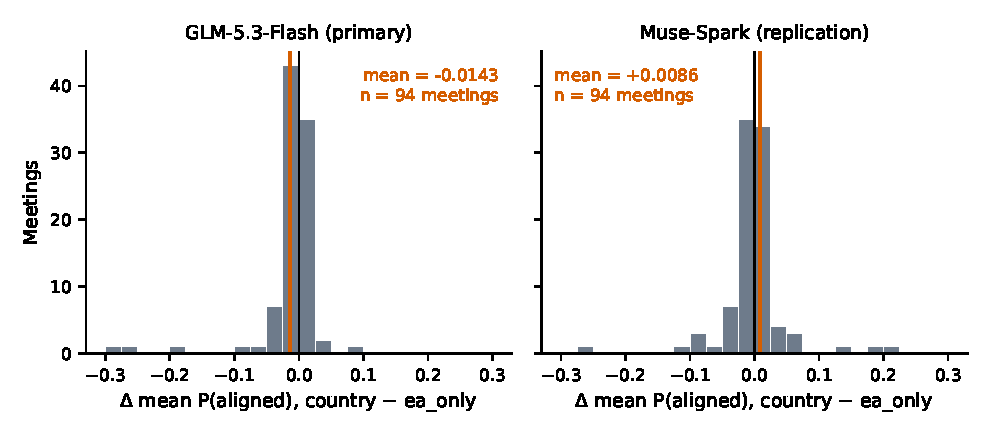
\includegraphics[width=\textwidth]{figures/fig2_arm_delta}
\caption{Distribution of the paired per-meeting treatment effect on estimated consensus, $\Delta = C^{\texttt{country}} - C^{\texttt{ea\_only}}$, in the two experiments. The black line marks zero; the orange line marks the mean. The distributions straddle zero in both experiments; the GLM mean is negative and the Muse mean positive, each within 1.5 percentage points of zero.}
\label{fig:delta}
\end{figure}

\subsection{Decision modes: above chance, but over-converging}\label{sec:modes}

Can the simulation recover \emph{how} the decision was reached? Table~\ref{tab:modes} compares simulated decision modes against the accounts ground truth. Match rates run 43--47 of 94 meetings (45.7--50.0\%), above the 37.2\% an always-unanimity classifier would achieve on this sample, and similar for the judge-based and deterministic aggregations. But the errors are not neutral. Panel~B shows the confusion matrix for the primary experiment: among the 39 meetings the accounts record as consensus, 28 are simulated as unanimity; the same skew appears in every experiment-arm-aggregator cell (23--34 of 39) and, more mildly, for majority meetings. The synthetic council converges more readily than the real one---deliberation among agents prompted to find common ground produces more agreement than the edited accounts report. Mode is also the softest outcome in the design: across generators, mode labels agree in only 58.5--63.8\% of meetings, against 95.7--97.9\% for decision stances. Figure~\ref{fig:cohesion} adds the time dimension: estimated cohesion is high throughout (0.83--0.97 yearly means) and dips in the same years under both generators---2019, 2020, and 2022, the years whose rate calls were closest.

\begin{table}[t]
\centering
\small
\caption{Decision-mode recovery against the accounts ground truth, and decision validity. Panel A: exact matches (of 94 meetings) for the judge-based and deterministic mode aggregations, and the share of simulated decisions matching the real decision's direction. Panel B: confusion matrix, judge-based modes, primary experiment, \texttt{ea\_only} arm; diagonal in bold, dominant error (ground-truth consensus simulated as unanimity) underlined.}
\label{tab:modes}
\begin{tabular}{llccc}
\toprule
\multicolumn{5}{l}{\textit{Panel A. Match rates and decision validity}} \\
Experiment & Arm & \multicolumn{2}{c}{Mode matches (of 94)} & Direction \\
\cline{3-4}
 & & Judge & Deterministic & accuracy \\
\midrule
GLM & \texttt{ea\_only}  & 43 & 44 & 0.957 \\
GLM & \texttt{country}   & 43 & 41 & 0.957 \\
Muse & \texttt{ea\_only} & 47 & 40 & 0.979 \\
Muse & \texttt{country}  & 45 & 37 & 0.957 \\
\midrule
\multicolumn{5}{l}{\textit{Panel B. Confusion matrix (GLM, \texttt{ea\_only}, judge)}} \\
 & \multicolumn{3}{c}{Simulated mode} & \\
\cline{2-4}
Accounts & Unanimity & Consensus & Majority & Total \\
\midrule
Unanimity & \textbf{29} & 5 & 1 & 35 \\
Consensus & \underline{28} & \textbf{9} & 2 & 39 \\
Majority & 10 & 5 & \textbf{5} & 20 \\
\bottomrule
\end{tabular}
\end{table}

\begin{figure}[t]
\centering
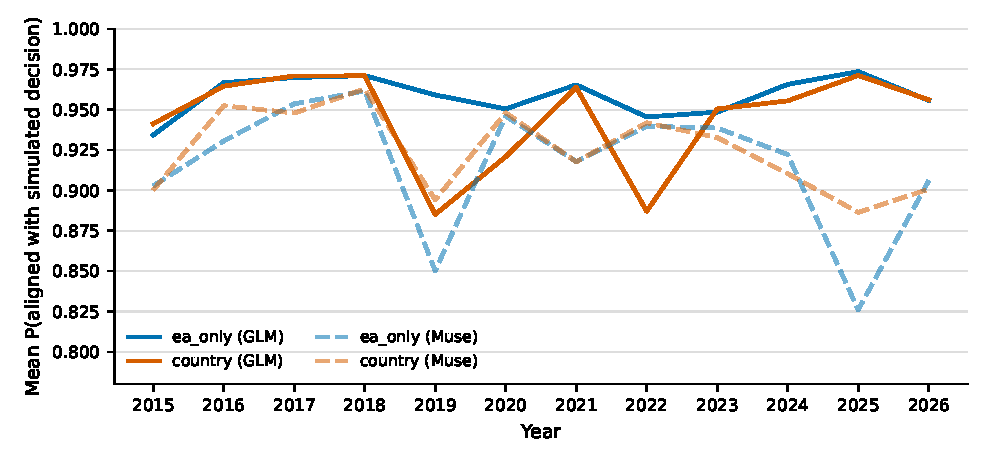
\includegraphics[width=\textwidth]{figures/fig3_cohesion}
\caption{Yearly mean estimated consensus by arm. Solid lines: primary experiment (GLM); dashed: replication (Muse). Levels differ across generators (a property of the apparatus, not the treatment); within each experiment the arms are indistinguishable. Cohesion dips in 2019, 2020, and 2022 under both generators.}
\label{fig:cohesion}
\end{figure}

\section{Discussion and limitations}\label{sec:discussion}

Three readings of the results. First, anchoring dominates. Once the verbatim proposal and the shared euro-area information set are in place, decisions replicate almost perfectly and are essentially invariant to the generator, the treatment, and the deliberation model. For forecasting decisions, the marginal value of a fancier simulation is small; the record does the work. Second, the country-information null is informative rather than empty. The heterogeneity literature documents that national conditions correlate with Council members' public positions; our experiment shows that \emph{adding} the national data to governors' information sets does not move the simulated deliberation. Reading the two together, the national-position correlations documented in administrative data may operate through priors and careers rather than through the current-data channel our treatment varies---or the deliberation protocol (public rounds, a consensus-seeking president) absorbs the additional dispersion. The ceiling compounds the power problem: baseline cohesion of 0.92--0.96 leaves little room to move, and any real effect of a seven-indicator table on a committee already holding euro-area staff projections is plausibly small. Third, consensus measurement is genuinely hard. The mode estimates beat chance, fail systematically toward unanimity, and disagree across generators far more than decisions do. Part of this is the target: the ground truth is itself a curated classification of edited accounts, not a transcript vote count. Part is the instrument: cohesion levels differ by generator, so only within-experiment contrasts are interpretable.

Four limitations bound the conclusions. The outcome is direction, not magnitude---the simulation says raise/hold/lower, not basis points. The sample is the accounts era (2015--2026); longer histories lack the anchor. All measurement flows through one judge family, albeit one returning calibrated probability distributions; the per-meeting ledgers allow replaying every measurement under a different judge without new generator calls, which we view as the natural robustness step. And the deliberation protocol is deliberately stylized---two rounds, alphabetical speaking order, a summarizing president---relative to the real Council's procedure.

The design points forward. Treatments that vary the \emph{strength} of national information (a shock narrative, not a table), weighting members by voting rights in the aggregation, and replaying measurement under alternative judges are all implementable on the existing artifacts at near-zero generator cost. The broader lesson for the LLM-simulation program in economics is methodological: a single-run simulation can produce a statistically significant, publishable-sounding effect---here, ``country information reduces consensus''---that a full replication under a different generator reveals as apparatus noise. Synthetic councils are cheap; the discipline of replicating them is what makes them evidence.

\section*{Data and code availability}

All data collectors, simulation code, prompts, per-meeting call ledgers, and analysis scripts are in the \texttt{synthetic-council} repository; every number in this paper is recomputable from the archived experiment artifacts (per-meeting parquets and settings-stamped comparison reports) via a single script.

\printbibliography

\end{document}
